\documentclass[11pt]{article}

\usepackage[letterpaper, margin=0.75in]{geometry}
\usepackage[utf8]{inputenc}
\usepackage[T1]{fontenc}
\usepackage[french]{babel}
\usepackage{graphicx}

\title{Travail pratique \#2 - IFT-2245}
\author{Jérémi Grenier-Berthiaumet et Olivier Lepage-Applin} 
\begin{document}

\maketitle

\section{Général}

La partie la plus longue et ennuyante du TP a été de s'assurer que le serveur soit robuste. Nous pensons que pour les prochaines itérations de ce TP, il serait préférable de ne pas faire en sorte que les étudiants aient à s'occuper de cela. S'assurer que le serveur puisse survivre à des requêtes pleines d'erreurs ou qui ne suivent pas le protocole présenté nous a semblé relativement inutile dans le cadre du cours: il y avait amplement de travail avec le reste. Établir un code de base qui fait fonctionner le protocole tel que présenté dans l'énoncé devrait être suffisant.

On pourrait aussi mentionner que plusieurs heures ont été passées à simplement observer le code afin de bien comprendre sa structure avant de commencer à jouer dans ses entrailles. De plus, l'énoncé semblait ambiguë et le protocole peut-être un peu mal défini, ce qui nous a fait perdre du temps pour réussir à savoir ce qui était attendu de nous en général. La structure du code donnait l'impression qu'on ne devait pas écrire du code à l'extérieur des endroits désignés par les "\texttt{TODO: BEGIN}" et "\texttt{TODO: END}": encore une fois du temps a été perdu afin de tenter de respecter ces bornes, avant de se faire confirmer qu'on pouvait en fait déborder. Par exemple, l'initialisation du serveur, du côté client, si on se restraignait aux bornes des \texttt{TODO}, nécessitait un \textit{mutex} ainsi qu'un booléen pour s'assurer qu'un seul des \textit{threads} client ne l'effectue. Ainsi, la confirmation qu'on pouvait modifier les \texttt{main} a changé notre approche en général (en plus de permettre de correctement \texttt{free} certaines structures qui y étaient déclarées, sans avoir à modifier la signature de certaines fonctions pour les passer en paramètre).

Toutefois, comparément au TP1, ce TP a tout de même eu l'avantage de ne pas requiérer autant de lecture de documentation. 

Finalement, nous avons désormais appris qu'il est possible d'éviter des \texttt{malloc} inutiles en passant en paramètre des pointeurs de variables déclarées localement à des fonctions et ce truc (qui nous aurait été fort utile dans le TP1) a été utilisé extensivement et a fortement facilité le passage du "test \texttt{valgrind}".


\section{Le Travail Pratique}

Certaines macros ont été utilisées pour augmenter la lisibilité et rapidité de changement durant le développement. Pensons par exemple à \texttt{PRINT\_EXTRACTED} qui s'occupe d'imprimer le contenu d'un \textit{array}.

Aussi, mentionnons qu'il a été apprécié de faire en sorte que l'utilisation correcte du \texttt{RNG} soit devenu un bonus puisque nous l'avions alors déjà implémenté.

Finalement, pour accélérer le développement, nous avons créer un petit "infographique" qui réusmait certains points du rapport pour avoir une référence rapide.

\begin{figure}
    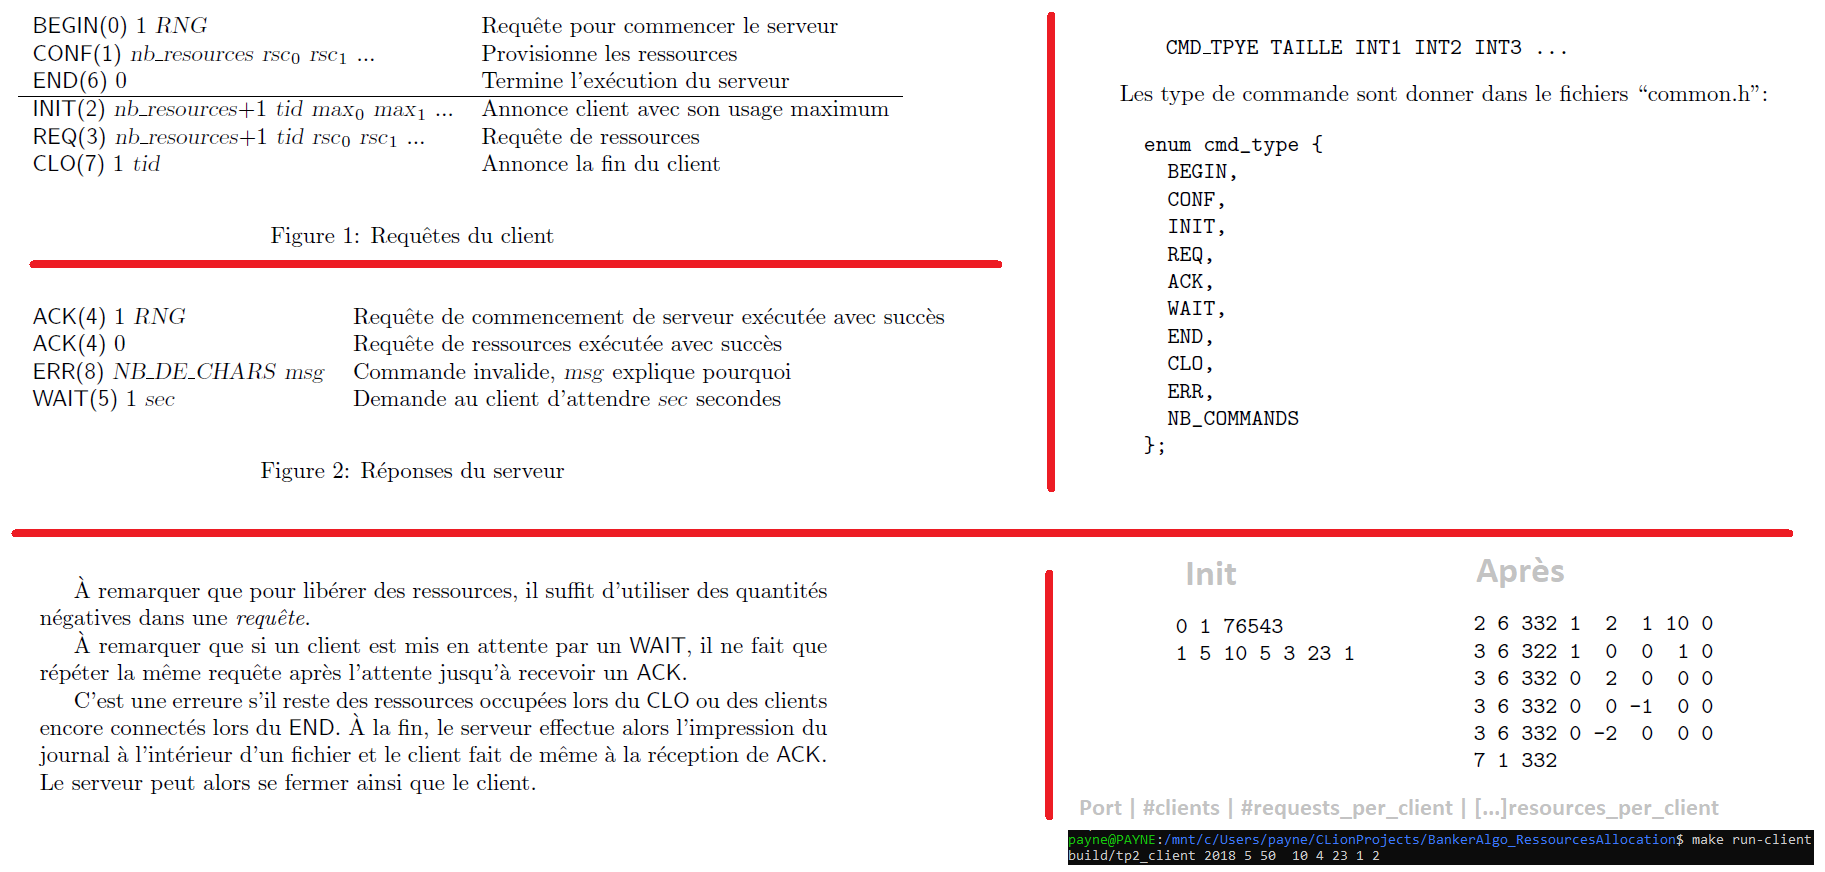
\includegraphics[width=\linewidth]{infographic.png}
    \caption{Notre infographique qui nous a été fort utile.}
    \label{fig:infog}
\end{figure}

\subsection{Sockets}

Il a été fortement apprécié d'avoir à notre disposition une fonction '\texttt{read\_socket}' mise à notre disposition. Cependant, nous avons tout de même eu à écrire nos propres fonctions pour s'occuper de l'écriture dans les sockets (l'envoie d'information). Ainsi, dans \texttt{common.c} nous avons ajouté \texttt{send\_header} et \texttt{send\_args}.

De plus, puisque le serveur pouvait envoyé des messages d'erreur (i.e. autre chose que des entiers), nous avons aussi ajouté dans \texttt{server\_thread.c} les fonctions \texttt{send\_msg} et \texttt{send\_err}. De façon générale, on utilise plutôt \texttt{send\_err} qui nous facilite la vie puisqu'on a alors qu'à passer une string (donc une chaîne de caractères terminée par un \texttt{NUL}).


\subsection{Mutex}

Nous avons implémenté un \textit{mutex} par "variable de statistique" (les compteurs affichés à la fin de l'exécution) afin de permettre une exécution plus indépendante des différents \textit{threads}. Si un unique \textit{mutex} avait été utilisé, le tout aurait tout de même fonctionné, mais le parallélisme aurait grandement été affecté négativement.


\subsection{Protocole}

On a utilisé \texttt{client\_thread->id} plutôt que le \textit{pt\_tid} pour les communications (le champ \textit{tid} des requêtes \texttt{INIT}, \texttt{REQ} et \texttt{CLO} des clients). Le fait que dans le cadre du TP cet \textit{id} soit monotone croissant nous a semblé suffisant pour justifier une telle approche et cela rendait le débuggage plus simple à effectuer.

Aussi, on a conservé la fonction qui ne reçoit que le header en premier puisque cela nous était fort utile pour déterminer la longueur
des arguments qui étaient à venir (ce qui est, en fait, essentiel puisque cela nous permet de connaître la grosseur du buffer à remplir par la fonction qui lit le contenu du socket).


\subsection{Algorithme du banquier}

Puisque l'algorithme est sensible aux changements des données associées aux clients, on ne pouvait pas se permettre de changer certaines variables durant son exécution. Pour cette raison, on a utilisé un \texttt{mutex\_lock} sur la variable \texttt{nb\_registered\_clients} avant de commencer l'algorithme pour ensuite le déverrouiller après l'exécution de l'algorithme. Cela ne fonctionnerait comme prévu que si nous utilisions aussi ce \textit{mutex} lors de l'enregistrement (\texttt{INIT}) et le désenregistrement (\textit{CLO}) des clients, ce qui a donc bien sûr été fait (on protège ainsi notre liste de clients, i.e. \texttt{clients\_list}, de façon générale).

La fonction \texttt{bankAlgo} est donc celle qui s'occupe d'exécuter l'algorithme. Les étapes décrites dans les notes de cours sont mises en évidence de façon approximative avec des commentaires du type \texttt{/* (Step 2) */}.

De plus, dans le terminal qui s'occupe de rouler le serveur, nous nous sommes arranger pour que l'envoie d'une commande \texttt{WAIT} ressorte visuellement parmi toutes les requêtes qui se déroulent rapidement devant vos yeux. En effet, vous allez pouvoir observer que la colonne de texte est généralement de la même largeur, sauf lorsque l'algorithme renvoie un \texttt{WAIT}: ce sont ces \textit{printf} de débuggage qui ressortent de temps en temps.

Finalement, il peut sembler que le tout s'exécute de façon séquentielle, mais en observant le début de l'exécution, on peut voir que ce n'est pas le cas: le parallélisme est bel et bien présent. C'est simplement qu'il y a de bonnes probabilités qu'un client soit "bloqué" relativement rapidement par une requête de sa part qui aurait été un peu trop "gourmande".


\subsection{Côté client}

Premièrement, tel que mentionné dans l'introduction, nous avons modifié le \texttt{main} afin de permettre au \textit{thread} principal de se comporter comme un client unique qui s'occupe de gérer l'initialisation du serveur avec les requêtes \texttt{BEGIN} et \texttt{CONF} dans la méthode "\texttt{ct\_init\_server}". Le booléen retourné correspond au succès ou non de cette initialisation et est utilisé pour gérer correctement les erreurs. En effet, si l'initialisation ne s'est pas bien passée, alors les différents \texttt{client\_thread} ne seront même pas initialisés et la procédure se termine.

Deuxièmement, un sémaphore a été utilisé afin de s'assurer d'éviter du \textit{busy wait} sur la variable \texttt{count} lorsque le \textit{main thread} arrive dans la méthode `\texttt{ct\_wait\_server}` après avoir instancié tous les \texttt{client\_thread} puisque cette instanciation utilise le \textit{flag} \texttt{PTHREAD\_CREATE\_DETACHED} et on ne pouvait donc pas tout simplement utiliser un \textit{join}. Ainsi, dans `\texttt{ct\_init\_server}` on s'occupe d'instancier le sémaphore et de l'initialiser à 0. De plus, à chaque fois qu'un \texttt{client\_thread} envoie sa requête \texttt{CLO} au serveur, il entre dans la méthode `\texttt{terminate\_client}` qui s'occupe de faire un \texttt{sem\_post}. De cette manière, on utilise ce signal dans une boucle \texttt{while} pour vérifier si le dernier client s'était bel et bien déconnecté.

Troisièmement, la signature de la fonction \texttt{send\_request} a été modifiée pour avoir accès au \textit{struct} `client\_thread`. Cela n'était pas nécessaire, mais rendait le tout plus "\textit{clean}".


\subsection{Côté serveur}

Une fois de plus, nous avons modifié le \texttt{main} afin de pouvoir gérer les cas d'erreur lors de l'établissement de la connection.

Aussi, tel que recommandé par un des démonstrateurs, nous avons utilisé un \textit{array} de fonction pour gérer de façon un peu plus élégante les différents comportements du serveur. Cependant, nous n'avons fait cela que pour une des phases du serveur, i.e. une fois qu'il est initialisé (donc que lorsqu'il s'attends à n'obtenir que des requêtes du type \texttt{REQ}/\texttt{CLO}/\texttt{END}).

La variable \texttt{nb\_registered\_clients} est utilisée pour s'assurer que tous les clients aient fait leur \texttt{CLO} avant d'accepter un appel à \texttt{END}. Nous renvoyons une erreur si jamais \texttt{END} est appelé sans que tous les clients se soient terminés.

Finalement, les variables de statistique en lien avec \texttt{REQ} sont légèrement ouvertes à l'interprétation. Pour notre part, par exemple, s'il y avait un nombre négatif qui indiquait le nombre d'arguments d'une requête \texttt{REQ}, celle-ci n'est pas réellement comptée. Cependant, si c'est un nombre d'argument positif mais qui ne correspond pas à \texttt{num\_resources + 1}, alors celle-ci est comptée comme une erreur.


\section{Varia}

Cette partie du rapport concerne les points que les démonstrateurs nous ont dit de spécifiquement mentionner dans le rapport ou sinon un simple rappel de ce qu'ils nous ont confirmés qui serait \textit{okay}.

Par rapport à la variable \texttt{request\_id} utilisée par les clients pour envoyer un certain nombre de requêtes fixé, nous avons décidé que le renvoie d'une requête causé par la réception d'un \texttt{WAIT} n'incrémenterait pas cette valeur.

Aussi, les démonstrateurs nous ont dit qu'il était correcte de simplement \texttt{exit} et de ne pas tenter de \texttt{free} lors d'une erreur sur \texttt{malloc}.

Un démonstrateur a aussi mentionné qu'il ne serait pas nécessaire de faire la vérification sur la variable de retour du \texttt{close(socket\_fd)}.

Nous ne considérons pas que la requête \texttt{CLO} fait partie du nombre de requêtes que devrait envoyer un client.

Certaines sections du code ont été enlevées (par exemple, la fonction \texttt{st\_signal}).

\end{document}
